% Provenance (never printed): see sources/outline_sources.md (Year 2: ancient massifs,
% Caledonian and Variscan belts; the Wilson cycle; supercontinents). Caledonian phases after
% McKerrow, Mac Niocaill and Dewey (2000) and Schiffer et al. (2020); the Wilson cycle after
% Chenin et al. (2018) and Schiffer et al. (2020); the Variscan belt after Faure (2024);
% supercontinents after Nance (2022); Siccar Point after the IUGS Geoheritage description.
% Model ocean and supercontinent chart from figdata/bachelor-2/wilson.py. Exercise and problem
% values in the Book 4 scratch calculator calc/ch15.py.
\chapter{Massifs anciens et cycle de Wilson}\label{ch:b2:wilson-cycle}

Sur la côte du sud-est de l'Écosse, à Siccar Point, des bancs de grès gris se dressent à la verticale
sous une couverture de grès rouge qui plonge doucement vers la mer. Les bancs gris se sont déposés
dans un océan au début du Silurien, puis ont été plissés et clivés lors de la fermeture de cet océan~;
ils ont été arasés en une surface irrégulière, puis des graviers rouges du Dévonien supérieur les ont
ensevelis, et une seconde orogenèse, plus douce, a incliné à son tour les couches rouges. Une falaise
témoigne d'un océan disparu, d'une chaîne de montagnes disparue et de la suivante. Ce chapitre lit de
tels témoignages, les rassemble en un cycle que suivent les bassins océaniques, et remonte au rythme
le plus long de tous, l'assemblage et la fragmentation des \omterm{def:b2:wilson-cycle:supercontinent}{supercontinents}.
% ledger: iugs:siccar-orogenies, iugs:siccar-point

\begin{recall}
\textbf{Des volumes scolaires~:} la Pangée et sa fragmentation, \omterm{def:b2:wilson-cycle:supercontinent}{supercontinents}~; discordances~;
le taux de dénudation, le rebond isostatique et la décroissance exponentielle d'une chaîne usée
par ses rivières. \textbf{Du volume de première année~:} rifts continentaux, marges passives et
dorsales médio-océaniques, vitesses d'expansion totale et demi-vitesse~; subduction et marges actives.
\textbf{Du \cref{ch:b2:crustal-melting} au \cref{ch:b2:himalaya-andes}}~: \omterm{def:b2:crustal-melting:migmatite}{migmatites} et
granites~; \omterm{def:b2:alpine-orogen:orogen}{orogène}, \omterm{def:b2:alpine-orogen:ophiolite}{ophiolite}, suture, \omterm{def:b2:alpine-orogen:nappes}{nappe de charriage}, \omterm{def:b2:alpine-orogen:foreland}{flysch} et \omterm{def:b2:alpine-orogen:foreland}{molasse}, \omterm{def:b2:alpine-orogen:foreland}{bassin d'avant-pays}~;
\omterm{def:b2:himalaya-andes:types}{orogènes de collision} et de type andin~; \omterm{def:b2:himalaya-andes:thickening}{épaississement crustal}, épaisseur d'Airy et \omterm{def:b2:himalaya-andes:collapse}{effondrement gravitaire}.
\end{recall}

\begin{omfigure}
\centering
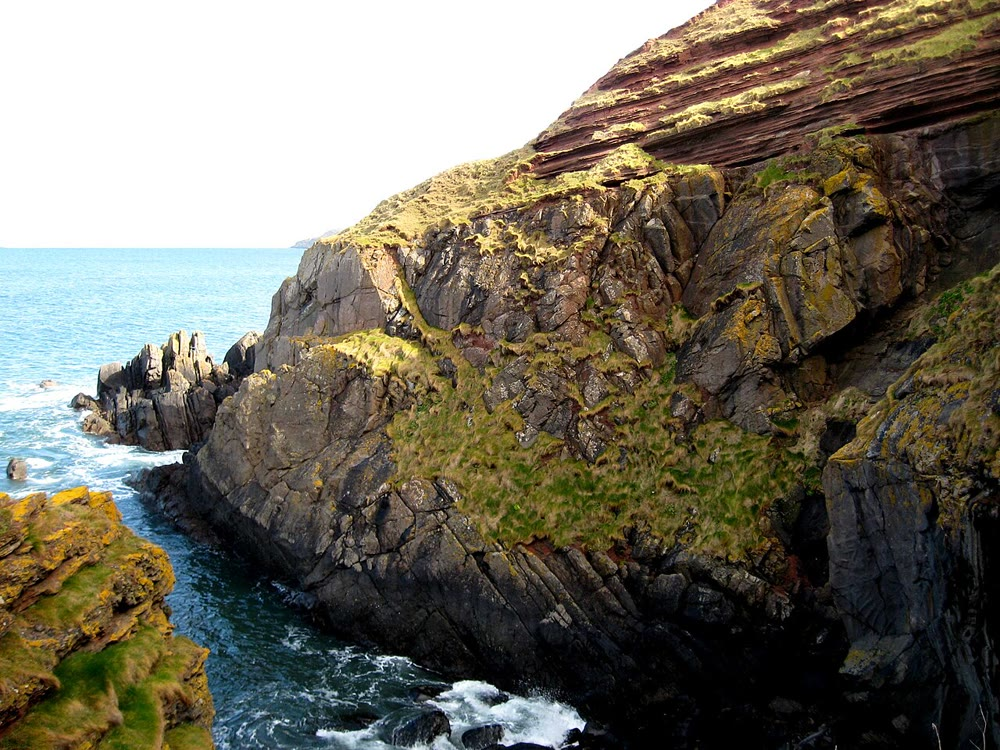
\includegraphics[width=0.64\linewidth]{images/book4/b2-15-siccar-point.jpg}
\par\smallskip{\small Siccar Point, au sud-est de la pointe~: bancs presque verticaux de grauwacke
silurienne grise, plissés lors de l'orogenèse calédonienne, sous des couches rouges faiblement inclinées
du Dévonien supérieur. Photographie de dave souza, 2008, CC BY-SA 4.0.}
\end{omfigure}
% ledger: iugs:siccar-orogenies

\section{Chaînes usées jusqu'à leurs racines}\label{sec:b2:wilson-cycle:old}

L'Europe occidentale et l'est de l'Amérique du Nord sont traversés par des chaînes de montagnes
bien plus anciennes que les Alpes. Leurs sommets ont disparu, mais leurs roches demeurent. Trois d'entre elles comptent ici.

La chaîne \emph{calédonienne} court de Norvège à travers l'Écosse et l'Irlande jusqu'à Terre-Neuve et
aux Appalaches du Nord, puis se prolonge par le Groenland oriental et le Svalbard. Elle garde la trace
d'un océan, l'Iapetus, qui occupait le Paléozoïque inférieur entre Laurentia, l'ancêtre de l'Amérique du Nord et
du Groenland, au nord-ouest, et Baltica et Avalonia, au sud-est et à l'est. Ses marges s'étaient disloquées
il y a environ 600~Ma~; sa fermeture, du Cambrien au
Dévonien, a produit une série entière de collisions, si bien que l'orogenèse calédonienne s'étale sur
près de 200~Ma. Le terme désigne un lieu et un océan, non un âge.
% ledger: mckerrow00:caledonian, schiffer20:caledonides

La chaîne \emph{varisque}, appelée hercynienne dans les anciens textes, traverse l'Europe depuis le
sud-ouest de l'Angleterre et la Belgique, à travers la France et l'Ibérie jusqu'en Europe centrale~; la chaîne \emph{appalachienne} de
l'est de l'Amérique du Nord en est la jumelle occidentale. Ensemble, elles enregistrent la fermeture des océans
entre le continent du sud, le Gondwana, et celui du nord, que les collisions calédoniennes venaient de souder
Leur dernière collision, au Carbonifère supérieur et au Permien, a laissé
une chaîne plissée orientée est--ouest à travers le sud de l'Europe, et nord-est--sud-ouest entre
l'est de l'Amérique du Nord et le nord-ouest de l'Afrique, et avec elle la Pangée.
% ledger: schiffer20:variscan, faure24:variscan

Comment reconnaître une chaîne de montagnes érodée depuis trois cents millions d'années~?
Non par son relief, qui a disparu. On cherche ses parties, chacune rencontrée par les
chapitres précédents~:
\begin{itemize}
\item \emph{sutures} bordées d'\emph{\omterm{def:b2:alpine-orogen:ophiolite}{ophiolites}}, lambeaux de plancher océanique d'un océan refermé~;
\item bandes de \emph{roches métamorphiques}, souvent de haut degré, racines de la croûte épaissie,
aujourd'hui à la surface parce que les kilomètres qui les recouvraient ont été érodés~;
\item \emph{granites} et \emph{\omterm{def:b2:crustal-melting:migmatite}{migmatites}}, produits de la fusion crustale que
entraînent l'épaississement et l'échauffement~;
\item sédiments de l'océan qui se referme et de la chaîne~: \emph{\omterm{def:b2:alpine-orogen:foreland}{flysch}} déposé dans des bassins profonds
pendant la convergence, \emph{\omterm{def:b2:alpine-orogen:foreland}{molasse}} déposée dans des \omterm{def:b2:alpine-orogen:foreland}{bassins d'avant-pays} et intramontagneux~;
\item \emph{discordances angulaires}, où des couches plus jeunes reposent sur des couches plissées et
érodées avant elles, qui datent la déformation entre les deux.
\end{itemize}

\begin{definition}[Pénéplaine]\label{def:b2:wilson-cycle:peneplain}
Une \emph{pénéplaine}\index{pénéplaine} est une surface continentale de faible relief, proche du niveau de base de
l'érosion, recoupant des roches de dureté et de structure différentes, par une longue érosion d'un ancien
relief.
\end{definition}

La chaîne varisque est un \omterm{def:b2:alpine-orogen:orogen}{orogène} chaud. Dans les Alpes du \cref{ch:b2:alpine-orogen}, les roches
suivaient des gradients métamorphiques d'environ \qty{8}{\celsius} par kilomètre~; dans la chaîne varisque,
d'environ \qty{30}{\celsius} par kilomètre. Sa croûte a largement fondu~: dans le Massif central
et le massif Armoricain, des \omterm{def:b2:crustal-melting:migmatite}{migmatites} se sont formées entre environ 330 et 325~Ma, et des
granites les ont intrudées. Cette fusion est la principale différence avec les Alpes occidentales. Lorsque la
collision s'achève, la croûte épaissie s'amincit par extension, des roches métamorphiques sont remontées
le long de détachements, et des bassins intramontagneux se sont ouverts~; puis l'érosion a aplani la chaîne en
une \omterm{def:b2:wilson-cycle:peneplain}{pénéplaine} permienne et triasique, sur laquelle se sont déposés les sédiments du cycle suivant.
% ledger: faure24:variscan

\begin{omfigure}
\centering\small
\begin{tabular}{>{\raggedright\arraybackslash}p{0.2\linewidth}|>{\raggedright\arraybackslash}p{0.17\linewidth}|>{\raggedright\arraybackslash}p{0.52\linewidth}}
phase & âge & ce qui est entré en collision \\ \hline
pénobscotienne & 490--485 Ma & un arc insulaire chevauché sur la marge avalonienne \\
grampienne, taconique & 480--455 Ma & arcs insulaires contre Laurentia (Écosse~; nord des Appalaches) \\
shelvienne & début de l'Ordovicien supérieur & Avalonia contre Baltica~; la mer de Tornquist se ferme \\
scandienne & 425--400 Ma & Baltica contre Laurentia~; les grandes \omterm{def:b2:alpine-orogen:nappes}{nappes de charriage} de Scandinavie \\
acadienne & Dévonien inférieur & des \omterm{def:b2:wilson-cycle:terrane}{terranes} venues du Gondwana contre le nouveau continent~; l'Iapetus est fermé \\
\end{tabular}
\par\smallskip{\small Principales phases de l'orogenèse calédonienne. Les phases précoces sont
des collisions d'arcs avec des arcs ou des continents, les phases tardives des collisions de continents~; la plupart
des phases ont commencé à des époques différentes selon les lieux.}
\end{omfigure}
% ledger: mckerrow00:phases, schiffer20:caledonides

Le tableau ci-dessus montre l'autre marque des vieilles chaînes~: elles sont composites. Avant que
deux continents ne se rencontrent, des arcs et des blocs plus petits arrivent un à un et sont soudés.

\begin{definition}[Terrane~; microcontinent]\label{def:b2:wilson-cycle:terrane}
Un \emph{terrane}\index{terrane} est un bloc de croûte délimité par des failles, dont l'histoire géologique diffère
de celle de ses voisins, amené à sa position actuelle par le mouvement des plaques~; il peut
être un arc insulaire, un plateau océanique, un lambeau de plancher océanique ou un fragment de continent. Un
\emph{microcontinent}\index{microcontinent} est un bloc de croûte continentale, plus petit
qu'un continent, séparé des continents par de la croûte océanique.
\end{definition}

Avalonia était un tel bloc~: une bande de croûte qui quitta la marge du Gondwana, ouvrit derrière elle l'océan Rhéique
à l'Ordovicien, traversa l'Iapetus et s'amarra contre Baltica, puis
Laurentia. L'Armorique et la Saxothuringe, aujourd'hui en France et en Allemagne, la suivirent tour à tour~; leurs
sutures, marquées par des \omterm{def:b2:alpine-orogen:ophiolite}{ophiolites}, découpent la chaîne varisque en zones, depuis un avant-pays
septentrional, sur l'ancien continent nord, jusqu'à un avant-pays méridional, sur le Gondwana.
% ledger: schiffer20:caledonides, schiffer20:variscan, faure24:variscan

\begin{omfigure}
\centering
\begin{tikzpicture}[x=0.5cm, y=0.5cm, font=\scriptsize]
\tikzset{cont/.style={fill=orange!25, draw=black!60, line width=0.4pt},
  terr/.style={fill=orange!45, draw=black!60, line width=0.4pt},
  ocn/.style={font=\scriptsize\itshape, text=blue!50!black},
  belt/.style={pattern=north east lines, pattern color=red!60!black, draw=red!60!black}}
% panel A
\begin{scope}
\fill[blue!6] (0,0) rectangle (9,8);
\draw[cont] (0.3,4.2) -- (3.0,4.0) -- (3.4,7.7) -- (0.3,7.7) -- cycle;
\node[align=center] at (1.7,6.0) {Lau-\\rentia};
\draw[cont] (6.0,5.4) -- (8.7,5.0) -- (8.7,7.7) -- (6.4,7.7) -- cycle;
\node at (7.4,6.6) {Baltica};
\draw[cont] (0.3,0.3) -- (8.7,0.3) -- (8.7,1.6) -- (0.3,1.9) -- cycle;
\node at (4.5,0.95) {Gondwana};
\draw[terr] (3.8,2.4) -- (6.6,2.2) -- (6.6,2.9) -- (3.8,3.1) -- cycle;
\node at (5.2,2.65) {Avalonia};
\node[ocn] at (4.6,5.4) {Iapetus};
\node[ocn] at (7.7,2.55) {Rhéique};
\node[anchor=north west, font=\small\bfseries] at (0.1,8.9) {A~: vers 480~Ma};
\end{scope}
% panel B
\begin{scope}[xshift=5.0cm]
\fill[blue!6] (0,0) rectangle (9,8);
\draw[cont] (0.3,3.6) -- (3.0,3.4) -- (3.4,7.7) -- (0.3,7.7) -- cycle;
\draw[cont] (3.0,3.4) -- (3.4,7.7) -- (8.7,7.7) -- (8.7,4.4) -- (5.2,4.6) -- (5.0,3.4) -- cycle;
\draw[terr] (3.0,3.4) -- (5.0,3.4) -- (5.2,4.6) -- (8.7,4.4) -- (8.7,3.6) -- (3.0,2.8) -- cycle;
\draw[red!60!black, line width=1.2pt] (3.0,3.4) -- (3.4,7.7);
\draw[red!60!black, line width=1.2pt] (5.0,3.4) -- (5.2,4.6) -- (8.7,4.4);
\node[align=center] at (1.6,5.6) {Lau-\\rentia};
\node at (6.6,5.7) {Baltica};
\node at (6.4,3.75) {Avalonia};
\node at (6.0,7.1) {\textbf{Laurussia}};
\draw[cont] (0.3,0.3) -- (8.7,0.3) -- (8.7,1.3) -- (0.3,1.5) -- cycle;
\node at (4.5,0.8) {Gondwana};
\draw[terr] (2.2,1.9) -- (3.6,1.9) -- (3.6,2.3) -- (2.2,2.3) -- cycle;
\draw[terr] (5.0,1.8) -- (6.6,1.8) -- (6.6,2.2) -- (5.0,2.2) -- cycle;
\node[ocn] at (7.7,2.3) {Rhéique};
\node[anchor=north west, font=\small\bfseries] at (0.1,8.9) {B~: vers 420~Ma};
\end{scope}
% panel C
\begin{scope}[xshift=10.0cm]
\fill[blue!6] (0,0) rectangle (9,8);
\draw[cont] (0.3,3.0) -- (8.7,3.0) -- (8.7,7.7) -- (0.3,7.7) -- cycle;
\draw[cont] (0.3,0.3) -- (8.7,0.3) -- (8.7,3.0) -- (0.3,3.0) -- cycle;
\fill[belt] (0.3,2.5) -- (8.7,2.5) -- (8.7,3.5) -- (0.3,3.5) -- cycle;
\node[fill=orange!25, inner sep=1pt] at (4.5,5.6) {Laurussia};
\node[fill=orange!25, inner sep=1pt] at (4.5,1.3) {Gondwana};
\node[fill=white, fill opacity=0.85, text opacity=1, inner sep=1pt, align=center] at (4.5,3.0)
  {chaîne varisque--appalachienne};
\node[ocn] at (7.6,0.7) {};
\node[anchor=north west, font=\small\bfseries] at (0.1,8.9) {C~: vers 300~Ma, la Pangée};
\end{scope}
\end{tikzpicture}
\par\smallskip{\small Trois moments de la fermeture des océans Iapetus et Rhéique, sous la forme d'une
esquisse schématique sans projection cartographique ni échelle~: positions, tailles et formes ne sont que
topologiques. A~: Avalonia a quitté le Gondwana et l'océan Rhéique s'ouvre derrière elle. B~: l'Iapetus s'est
refermé~; Laurentia, Baltica et Avalonia forment Laurussia, le long de sutures calédoniennes (en rouge)~;
de petits blocs traversent l'océan Rhéique. C~: le Gondwana a rencontré Laurussia le long de la
chaîne varisque--appalachienne (hachurée).}
\end{omfigure}
% ledger: mckerrow00:caledonian, mckerrow00:phases, schiffer20:caledonides, schiffer20:variscan, faure24:variscan

\section{Le cycle de Wilson}\label{sec:b2:wilson-cycle:cycle}

En 1966, J. Tuzo Wilson se demanda si l'Atlantique s'était d'abord refermé, puis
rouvert. Des fossiles du Paléozoïque inférieur et moyen lui apprirent qu'un vaste océan séparait alors
les faunes d'Amérique du Nord de celles de l'Europe occidentale, un océan qui n'existait plus du
Paléozoïque supérieur au milieu du Mésozoïque. L'Atlantique actuel s'était ouvert presque
à l'endroit où s'était refermé cet ancien océan, l'Iapetus.
% ledger: schiffer20:wilson, chenin18:cycle

\begin{definition}[Cycle de Wilson]\label{def:b2:wilson-cycle:wilson}
Le \emph{cycle de Wilson}\index{cycle de Wilson} est la succession des étapes par lesquelles un bassin océanique
s'ouvre puis se referme entre des marges continentales~: rifting continental, fragmentation et
expansion océanique, océan élargi à marges passives, début de la
subduction, rétrécissement et fermeture de l'océan, collision continentale, effondrement
et érosion de la chaîne, après quoi le continent ressoudé peut de nouveau se disloquer le long de la même zone.
\end{definition}

La figure ci-dessous suit ces étapes. Ce sont celles des chapitres précédents, mises en ordre~:
les rifts et marges passives du volume de première année, les marges actives et leurs arcs, les
collisions alpine et himalayenne, l'\omterm{def:b2:himalaya-andes:collapse}{effondrement gravitaire} du Tibet, l'usure lente
des vieilles chaînes.

\begin{omfigure}
\centering
\begin{tikzpicture}[x=0.38cm, y=0.38cm, font=\scriptsize]
\tikzset{crust/.style={fill=orange!25, draw=black!60, line width=0.3pt},
  ocrust/.style={fill=gray!45, draw=black!60, line width=0.3pt},
  sea/.style={fill=blue!8},
  ttl/.style={anchor=west, font=\scriptsize\bfseries}}
% 1 continent
\begin{scope}
\draw[crust] (0,0) -- (16,0) -- (16,2) -- (0,2) -- cycle;
\node[ttl] at (0,3.1) {1\enspace un continent};
\end{scope}
% 2 rift
\begin{scope}[xshift=7.2cm]
\draw[crust] (0,0) -- (7,0) -- (7,2) -- (6.2,2) -- (5.4,1.0) -- (0,2) -- cycle;
\draw[crust] (9,0) -- (16,0) -- (16,2) -- (10.6,1.0) -- (9.8,2) -- (9,2) -- cycle;
\fill[red!50] (7,0) -- (9,0) -- (8.6,1.2) -- (7.4,1.2) -- cycle;
\draw[thick] (6.2,2) -- (7,0.4); \draw[thick] (9.8,2) -- (9,0.4);
\node[ttl] at (0,3.1) {2\enspace rift};
\end{scope}
% 3 young ocean
\begin{scope}[yshift=-2.4cm]
\fill[sea] (5,2) -- (11,2) -- (11,0.6) -- (5,0.6) -- cycle;
\draw[crust] (0,0) -- (5,0) -- (6.2,0.5) -- (5,2) -- (0,2) -- cycle;
\draw[crust] (16,0) -- (11,0) -- (9.8,0.5) -- (11,2) -- (16,2) -- cycle;
\draw[ocrust] (6.2,0.5) -- (9.8,0.5) -- (9.8,0) -- (6.2,0) -- cycle;
\draw[red!70!black, thick] (8,0.5) -- (8,1.0);
\node[ttl] at (0,3.1) {3\enspace un océan jeune};
\end{scope}
% 4 wide ocean
\begin{scope}[xshift=7.2cm, yshift=-2.4cm]
\fill[sea] (2.5,2) -- (13.5,2) -- (13.5,0.4) -- (2.5,0.4) -- cycle;
\draw[crust] (0,0) -- (2.5,0) -- (3.4,0.4) -- (2.5,2) -- (0,2) -- cycle;
\draw[crust] (16,0) -- (13.5,0) -- (12.6,0.4) -- (13.5,2) -- (16,2) -- cycle;
\draw[ocrust] (3.4,0.4) -- (12.6,0.4) -- (12.6,-0.4) -- (3.4,-0.4) -- cycle;
\draw[red!70!black, thick] (8,0.4) -- (8,0.9);
\node[anchor=north] at (3,-0.1) {passive};
\node[anchor=north] at (13,-0.1) {passive};
\node[ttl] at (0,3.1) {4\enspace un océan large};
\end{scope}
% 5 subduction begins
\begin{scope}[yshift=-4.8cm]
\fill[sea] (2.5,2) -- (13.5,2) -- (13.5,0.4) -- (2.5,0.4) -- cycle;
\draw[crust] (0,0) -- (2.5,0) -- (3.4,0.4) -- (2.5,2) -- (0,2) -- cycle;
\draw[crust] (16,-0.4) -- (13.3,-0.4) -- (12.6,0.4) -- (13.5,2) -- (16,2) -- cycle;
\draw[ocrust] (3.4,0.4) -- (12.6,0.4) -- (11.6,-1.6) -- (3.4,-0.4) -- cycle;
\fill[red!60!black] (14.2,2) -- (14.6,2.7) -- (15.0,2) -- cycle;
\draw[red!70!black, thick] (7,0.4) -- (7,0.9);
\node[anchor=north] at (13.5,-0.5) {fosse};
\node[ttl] at (0,3.1) {5\enspace début de la subduction};
\end{scope}
% 6 ocean closes
\begin{scope}[xshift=7.2cm, yshift=-4.8cm]
\fill[sea] (5.5,2) -- (10.5,2) -- (10.5,0.4) -- (5.5,0.4) -- cycle;
\draw[crust] (0,0) -- (5.5,0) -- (6.4,0.4) -- (5.5,2) -- (0,2) -- cycle;
\draw[crust] (16,-0.4) -- (11.3,-0.4) -- (10.6,0.4) -- (11.5,2.4) -- (16,2.4) -- cycle;
\draw[ocrust] (6.4,0.4) -- (10.6,0.4) -- (9.4,-1.8) -- (6.4,-0.4) -- cycle;
\fill[red!60!black] (12.4,2.4) -- (12.8,3.1) -- (13.2,2.4) -- cycle;
\node[anchor=north west] at (11.6,-0.5) {arc, fosse};
\node[ttl] at (0,3.1) {6\enspace l'océan se referme};
\end{scope}
% 7 collision
\begin{scope}[yshift=-7.2cm]
\draw[crust] (0,0) -- (16,0) -- (16,2) -- (10,2) -- (8.6,3.6) -- (7.4,3.4) -- (6,2) -- (0,2) -- cycle;
\fill[crust] (5.6,0) -- (10.4,0) -- (9.6,-1.6) -- (6.4,-1.6) -- cycle;
\draw[black!60, line width=0.3pt] (5.6,0) -- (6.4,-1.6) -- (9.6,-1.6) -- (10.4,0);
\draw[red!60!black, line width=1pt] (8.6,3.6) -- (7.6,-1.6);
\node[anchor=west, text=red!60!black] at (9.0,3.5) {suture};
\node[ttl] at (0,3.1) {7\enspace collision};
\end{scope}
% 8 worn flat
\begin{scope}[xshift=7.2cm, yshift=-7.2cm]
\draw[crust] (0,0) -- (16,0) -- (16,2) -- (0,2) -- cycle;
\draw[red!60!black, line width=1pt] (8.4,2) -- (7.6,0);
\fill[pink!60!red!40] (6.0,1.0) ellipse (0.7 and 0.4);
\node[anchor=north] at (8,-0.1) {pénéplaine sur l'ancienne racine};
\node[ttl] at (0,3.1) {8\enspace une chaîne aplanie~; un rifting peut suivre};
\end{scope}
\end{tikzpicture}
\par\smallskip{\small Les étapes du \omterm{def:b2:wilson-cycle:wilson}{cycle de Wilson}, en coupes schématiques (sans échelle)~:
croûte continentale en orange, croûte océanique en gris, la dorsale en rouge, volcans de l'arc en
triangles~; dans le dernier panneau, la suture et un granite subsistent dans une croûte d'épaisseur normale.}
\end{omfigure}
% ledger: chenin18:cycle, schiffer20:wilson

\subsection{Quelle largeur, quelle durée~?}

Un océan s'élargit par expansion océanique à sa dorsale et se rétrécit par subduction à ses fosses.
Un simple bilan donne sa largeur.

\begin{proposition}[Largeur d'un océan au cours d'un cycle]\label{prop:b2:wilson-cycle:width}
Supposons qu'un océan s'ouvre à l'instant $t_0$ et s'élargisse à la vitesse d'expansion totale $V_s$ de sa
dorsale, jusqu'à ce qu'une zone de subduction commence à une marge à l'instant $t_1$ et consomme du plancher océanique à la vitesse $V_c$
par rapport à cette marge, avec $V_c > V_s$, la dorsale continuant de s'étendre. Sa largeur est
\[
  W(t) = V_s\,(t - t_0) \quad (t_0 \le t \le t_1), \qquad
  W(t) = V_s\,(t_1 - t_0) - (V_c - V_s)\,(t - t_1) \quad (t \ge t_1),
\]
maximale à $t_1$, et l'océan se referme un temps $V_s(t_1 - t_0)/(V_c - V_s)$ après le début de la
subduction. Avec une expansion symétrique, la dorsale se déplace vers la fosse à $V_c - V_s/2$.
\end{proposition}

\begin{proof}
Fixons la marge, la fosse restant immobile. Avant $t_1$, les deux marges s'écartent à pleine
vitesse $V_s$, si bien que la largeur croît à $V_s$ à partir de zéro. Après $t_1$, la plaque située entre
la fosse et la dorsale se dirige vers la fosse à $V_c$~; la dorsale ajoute $V_s$ à la distance
entre cette plaque et la plaque éloignée, si bien que la marge éloignée se dirige vers la fosse à $V_c - V_s$,
la vitesse à laquelle la largeur diminue. La largeur s'annule après $V_s(t_1 - t_0)/(V_c -
V_s)$. Avec une expansion symétrique, la dorsale se déplace à la moyenne des vitesses des plaques de
part et d'autre, $(V_c + (V_c - V_s))/2 = V_c - V_s/2$.
\end{proof}

La figure ci-dessous déroule ce bilan pour un océan modèle de type Iapetus~: expansion à partir de
\qty{570}{Ma} à \qty{30}{mm} par an, subduction à partir de \qty{490}{Ma} consommant \qty{60}{mm}
par an. Ces vitesses sont des hypothèses, des valeurs rondes de l'ordre de celles qu'on mesure aujourd'hui dans les océans~; le
véritable Iapetus n'était ni si simple ni si bien connu. L'océan modèle atteint \qty{2400}{km}
et se referme à \qty{410}{Ma}, dans l'intervalle de temps de la collision scandienne.
% values (wilson.py): max_width_km 2400, closure_Ma 410; ledger: mckerrow00:caledonian, schiffer20:caledonides

\begin{omfigure}
\centering
% figdata/bachelor-2/wilson.py part ocean (model values: assumptions)
\begin{tikzpicture}
\begin{axis}[width=0.8\linewidth, height=5.0cm, x dir=reverse, xmin=360, xmax=600, ymin=0,
  ymax=3300, ytick={0,1000,2000,3000}, xlabel={âge (\unit{Ma})}, ylabel={largeur de l'océan (\unit{km})},
  tick label style={font=\scriptsize}, label style={font=\small}, xtick={600,560,...,360}]
\addplot[omThm, line width=1.2pt] table[x=t_Ma, y=width_km] {figdata/out/bachelor-2-wilson-ocean.dat};
\draw[dashed, black!50] (axis cs:490,0) -- (axis cs:490,2400);
\draw[dashed, black!50] (axis cs:570,0) -- (axis cs:570,2750);
\draw[dashed, black!50] (axis cs:410,0) -- (axis cs:410,2750);
\node[font=\scriptsize, anchor=south] at (axis cs:570,2750) {début de l'expansion};
\node[font=\scriptsize, anchor=south west] at (axis cs:488,2400) {début de la subduction};
\node[font=\scriptsize, anchor=south] at (axis cs:410,2750) {collision};
\node[font=\scriptsize, anchor=west] at (axis cs:540,600) {ouverture à $V_s$};
\node[font=\scriptsize, anchor=south west, align=left] at (axis cs:446,1150) {fermeture\\à $V_c - V_s$};
\end{axis}
\end{tikzpicture}
\par\smallskip{\small Largeur d'un océan modèle au cours d'un \omterm{def:b2:wilson-cycle:wilson}{cycle de Wilson}, d'après
la \cref{prop:b2:wilson-cycle:width} avec $V_s = \qty{30}{mm}$ par an à partir de \qty{570}{Ma} et $V_c
= \qty{60}{mm}$ par an à partir de \qty{490}{Ma}. Le temps croît de gauche à droite.}
\end{omfigure}

\subsection{Ouvrir là où il s'était refermé}

L'idée de Wilson repose sur un principe mécanique~: une vieille chaîne est une zone faible, et un continent
que l'on écarte tend à se rompre le long de ses zones faibles plutôt qu'à travers son
intérieur fort et stable.

\begin{definition}[Réactivation structurale]\label{def:b2:wilson-cycle:reactivation}
La \emph{réactivation structurale}\index{réactivation structurale} d'une structure préexistante
(faille, zone de cisaillement, suture, contact lithologique) est la concentration renouvelée
de la déformation le long de celle-ci, sous un champ de contraintes ultérieur qui peut différer de celui qui l'a formée.
\end{definition}

L'Atlantique Nord est le cas d'école, et il ne se vérifie qu'en partie. Dans l'Atlantique central, le
jeune océan suit de près les Appalaches. Entre la Scandinavie et le Groenland, la fragmentation
suit largement la chaîne calédonienne. Plus au sud, ce n'est pas le cas~: la suture de l'Iapetus traverse encore
le nord de l'Angleterre et le centre de l'Irlande, et l'Atlantique s'est ouvert à l'ouest, laissant
des morceaux de l'ancienne croûte de Laurentia sur la marge nord-ouest de l'Europe, autour de Rockall et de Hatton.
Plus au nord-ouest, la mer du Labrador et la baie de Baffin recoupent en droite ligne des cratons et des
chaînes plus anciennes. Les vieilles structures guident les rifts ultérieurs, mais pas toujours~: une faiblesse refroidie depuis plus de
30 à 50~Ma peut être devenue résistante, et un nouveau rift peut suivre la fabrique plus profonde
du manteau plutôt que la suture crustale. Le \omterm{def:b2:wilson-cycle:wilson}{cycle de Wilson} est un guide, non une loi.
% ledger: schiffer20:wilson, schiffer20:reactivation

Tous les cycles n'ouvrent pas un océan large. Beaucoup d'\omterm{def:b2:alpine-orogen:orogen}{orogènes} ferment des océans embryonnaires, des rifts à peine
ouverts à l'expansion, d'une largeur inférieure à environ \qty{500}{km}~: les Alpes, les Pyrénées, la plus grande partie de
la chaîne varisque d'Europe occidentale. D'autres ferment de larges océans matures, comme les
Calédonides scandinaves. La différence apparaît à la fin~: une chaîne qui a fermé un océan large portait un
arc de longue durée, qui a vidé le manteau sous-jacent de sa partie fusible~; son effondrement fut pauvre en
\omterm{def:b2:magma-emplacement:magma}{magma}, comme dans les Calédonides. Une chaîne qui a fermé un bassin étroit repose sur un \omterm{def:b2:mantle-melting:fertility}{manteau fertile}~; son
effondrement peut être riche en \omterm{def:b2:magma-emplacement:magma}{magma}, comme dans la chaîne varisque, où le Moho est aujourd'hui plat et la
croûte inférieure stratifiée, lue comme du basalte sous-plaqué sous la croûte, ou comme une croûte inférieure
cisaillée pendant qu'elle était chaude. En quelques dizaines de Ma, les anomalies
thermiques d'une chaîne s'estompent~; ses structures demeurent.
% ledger: chenin18:cycle

\section{Supercontinents}\label{sec:b2:wilson-cycle:supercontinents}

\begin{definition}[Supercontinent~; cycle des supercontinents]\label{def:b2:wilson-cycle:supercontinent}
Un \emph{supercontinent}\index{supercontinent} est une masse continentale qui rassemble la plus grande part de la
croûte continentale terrestre en un seul bloc. Le \emph{cycle des supercontinents}\index{cycle des supercontinents}
est l'assemblage épisodique des continents en un supercontinent, suivi de sa
fragmentation ultérieure, répétée au fil de l'histoire de la Terre.
\end{definition}

La Pangée, que Wegener a reconstituée et que les volumes scolaires ont décrite, a existé d'environ 325
à 200~Ma. D'autres \omterm{def:b2:wilson-cycle:supercontinent}{supercontinents} ont été proposés~: Pannotia, vers 620 à
580~Ma, dont l'existence est discutée~; Rodinia, vers 950 à 800~Ma~;
Nuna, aussi appelé Columbia, vers 1.6 à 1.4~Ga~; et, plus douteux, Kenorland
vers 2.7 à 2.5~Ga, et Ur vers 3.0~Ga. Ils semblent s'être assemblés et fragmentés à des
intervalles d'environ 500~Ma depuis peut-être la fin de l'Archéen. Le cycle a été relié aux
âges des orogenèses, aux pics d'âge des granites et des grains de zircon qu'ils contiennent,
à la croissance de la croûte, aux grandes provinces magmatiques, au niveau de la mer et au
climat~: l'assemblage d'un \omterm{def:b2:wilson-cycle:supercontinent}{supercontinent} tend à coïncider
avec un refroidissement.
% ledger: nance22:supercontinents

\begin{omfigure}
\centering
% figdata/bachelor-2/wilson.py part supercontinents; ledger: nance22:supercontinents
\begin{tikzpicture}
\begin{axis}[width=0.86\linewidth, height=4.6cm, x dir=reverse, xmin=0, xmax=3300, ymin=-0.7,
  ymax=6.5, ytick=\empty, xlabel={âge (\unit{Ma})}, tick label style={font=\scriptsize},
  label style={font=\small}, xtick={0,500,...,3000}, axis y line*=left,
  % étiquettes : nœuds explicites (la table figdata porte les noms anglais)
  clip=false]
\addplot[only marks, mark=*, mark size=1.6pt, omThm,
  error bars/.cd, x dir=both, x explicit, error bar style={line width=3pt, omThm!60}, error mark=none]
  table[x=mid_Ma, y=row, x error=half_Ma] {figdata/out/bachelor-2-wilson-supercontinents.dat}; \foreach \x/\y/\n in {3000/0/Ur, 2600/1/Kenorland, 1500/2/Nuna-Columbia, 875/3/Rodinia, 600/4/Pannotia, 262.5/5/Pangée} {\edef\temp{\noexpand\node[font=\noexpand\scriptsize, anchor=south, yshift=2pt] at (axis cs:\x,\y) {\n};}\temp}
\end{axis}
\end{tikzpicture}
\par\smallskip{\small \omterm{def:b2:wilson-cycle:supercontinent}{Supercontinents} au fil de l'histoire de la Terre, de l'assemblage à la
fragmentation, datés d'après une revue récente~: les barres couvrent les intervalles cités (Ur ne donne qu'une estimation), les
points marquent leurs milieux. Pannotia, Kenorland et Ur sont discutés. Le temps croît de gauche à droite.}
\end{omfigure}

Le cycle est-il vraiment périodique~? Les milieux des intervalles du graphique sont séparés de 400,
1100, 625, 275 et 337.5~Ma~: en moyenne environ 550, mais dispersés d'un facteur
quatre. «~Environ un demi-milliard d'années~» est une tendance, non une horloge, et les
\omterm{def:b2:wilson-cycle:supercontinent}{supercontinents} plus anciens reposent sur des indices ténus.
% values (wilson.py): spacings 400 1100 625 275 337.5, mean 547.5 Myr

\section{Des montagnes aux plaines}\label{sec:b2:wilson-cycle:erosion}

Qu'est-ce qui transforme une chaîne comme l'Himalaya en collines basses de Bretagne~? Le volume scolaire
a construit un modèle~: les rivières usent une chaîne à une vitesse proportionnelle à son altitude moyenne, $kh$,
et chaque mètre retiré du sommet est en partie restitué par le rebond isostatique, si bien que seule
la fraction $f = (\rho_m - \rho_c)/\rho_m$ de cette masse est perdue sous forme de hauteur. L'altitude moyenne décroît alors
selon
\[
  h(t) = h_0\,e^{-k f t} ,
\]
avec le temps caractéristique $\tau = 1/(kf)$. Dans les grands bassins de latitude moyenne, le taux de dénudation est
proportionnel au relief moyen et, sans soulèvement, le relief tomberait au dixième de sa
valeur en environ 11~Ma~: $k = \ln 10/11 \approx 0.21$ par Ma. Avec les
masses volumiques 2700 et \qty{3300}{kg.m^{-3}}, $f = 0.18$ et $\tau \approx \qty{26}{Ma}$~: une
chaîne haute de \qty{3}{km} se dresse encore à \qty{1}{km} de hauteur environ 30~Ma plus tard, et
s'abaisse sous \qty{300}{m} après environ 60~Ma.
% ledger: ahnert70:decay; values (wilson.py): k 0.20933 /Myr, f 0.18182, tau 26.275 Myr

Le même rebond explique pourquoi les vieilles chaînes exposent leurs racines. Pour ramener une croûte épaissie de
$H$ à $T$ au niveau de la mer, toute l'épaisseur en excès $T - H$ doit être érodée, alors que l'altitude moyenne
n'était que $(T - H)f$~: environ 5.5 fois plus de roche est enlevée que la hauteur de la
chaîne. Les roches qui étaient à 20 ou \qty{30}{km} de profondeur dans la racine remontent à la surface~: les
\omterm{def:b2:crustal-melting:migmatite}{migmatites}, granites et gneiss de haut degré des vieux massifs, comme ceux du Massif
central.
% ledger: ahnert70:decay

La chaîne varisque, dont les dernières collisions ont pris fin vers 290~Ma, avait été
aplanie en \omterm{def:b2:wilson-cycle:peneplain}{pénéplaine} pendant le Permien et le Trias, en une soixantaine de Ma, ce que donne le
modèle. L'effondrement peut accélérer le processus~: l'extension d'une croûte épaissie, comme
Tibet aujourd'hui, l'amincit directement, sans attendre les rivières. À Siccar Point, des graviers du Dévonien supérieur reposent sur
des couches siluriennes plissées lors des collisions calédoniennes, sur une ancienne surface émergée qui conserve
un certain relief entre les couches dures et les couches tendres.
% ledger: faure24:variscan, iugs:siccar-orogenies

\begin{inthefield}[Lire une discordance angulaire]
Les géologues qui étudient une discordance angulaire comme celle de Siccar Point commencent par mesurer
l'attitude des couches situées sous et au-dessus de la surface, direction et pendage, en de nombreux endroits. Ils cherchent
la polarité des couches inférieures, grâce au granoclassement ou aux marques de base des couches,
car des couches plissées peuvent être renversées. Ils examinent la surface elle-même~: son relief, les
altérations sous-jacentes, les galets des roches plus anciennes dans le conglomérat qui la recouvre. Puis ils
datent~: les fossiles les plus jeunes situés en dessous donnent l'âge avant lequel le plissement n'a pu se produire,
les fossiles les plus anciens situés au-dessus donnent l'âge avant lequel il avait eu lieu et le terrain avait été
érodé. L'intervalle entre les deux bornes encadre l'orogenèse. À Siccar Point, les couches inférieures sont du
Silurien inférieur et les supérieures du Dévonien supérieur, et le plissement, le soulèvement et l'érosion calédoniens
s'insèrent entre les deux~; l'inclinaison douce des couches supérieures est plus récente encore, varisque.
\end{inthefield}
% ledger: iugs:siccar-orogenies, ics:base.Silurian, ics:base.Devonian, ics:base.Carboniferous

\section*{Exercices}\label{sec:b2:wilson-cycle:exercises}

Données~: $g = \qty{9.8}{m.s^{-2}}$~; masses volumiques de la croûte et du manteau
\qty{2700}{kg.m^{-3}} et \qty{3300}{kg.m^{-3}}~; croûte normale $H = \qty{35}{km}$~; âges des
bases du Silurien, du Dévonien et du Carbonifère, 443.1, 419.6 et \qty{358.9}{Ma}, du
Trias \qty{251.9}{Ma}.

\begin{exercise}[$\star$]\label{exo:b2:wilson-cycle:1}
Les marges de l'Iapetus se sont disloquées vers \qty{600}{Ma}~; la principale collision calédonienne, la
scandienne, s'est achevée vers \qty{400}{Ma}~; la première collision arc--continent avec Laurentia a commencé
vers \qty{480}{Ma}. (a) Combien de temps a duré l'ensemble du cycle de l'Iapetus~? (b) Combien de temps ont duré les
collisions~? (c) Pourquoi ne faut-il pas employer «~calédonien~» pour désigner un âge~?
\end{exercise}

\begin{exercise}[$\star$]\label{exo:b2:wilson-cycle:2}
Ranger ces situations dans l'ordre du \omterm{def:b2:wilson-cycle:wilson}{cycle de Wilson} et nommer l'étape de chacune~: (a) la mer Rouge,
un océan étroit entre de jeunes marges en rifting~; (b) l'Himalaya~; (c) le
rift est-africain~; (d) l'océan Atlantique, large, à marges passives des deux côtés~; (e) la marge pacifique
de l'Amérique du Sud~; (f) les basses collines de Bretagne sur un socle ancien de granite et de gneiss.
\end{exercise}

\begin{exercise}[$\star$]\label{exo:b2:wilson-cycle:3}
À Siccar Point, des couches du Silurien inférieur reposent sous des couches du Dévonien supérieur. (a) Entre quelles bornes,
données ci-dessus, le plissement, le soulèvement et l'érosion ont-ils dû se produire~? (b) Quelle est
la durée maximale qu'ils ont pu prendre~? (c) Énumérer dans l'ordre les événements que la falaise enregistre.
\end{exercise}

\begin{exercise}[$\star$]\label{exo:b2:wilson-cycle:4}
Dire si chacun est un \omterm{def:b2:wilson-cycle:terrane}{terrane}, un \omterm{def:b2:wilson-cycle:terrane}{microcontinent}, les deux ou aucun, et pourquoi~: (a) Avalonia~;
(b) Laurentia~; (c) un arc insulaire accolé à un continent~; (d) la suture de l'Iapetus.
\end{exercise}

\begin{exercise}[$\star\star$]\label{exo:b2:wilson-cycle:5}
Prendre les milieux des intervalles des \omterm{def:b2:wilson-cycle:supercontinent}{supercontinents} Ur (3000), Kenorland (2600),
Nuna (1500), Rodinia (875), Pannotia (600) et la Pangée (262.5), exprimés en Ma.
(a) Calculer les cinq écarts et leur moyenne. (b) Quel est le rapport de l'écart le plus grand à
le plus petit~? (c) Retirer Kenorland et Ur, douteux~: quel est l'écart moyen des
quatre autres~? «~un demi-milliard d'années~» est-il une période~?
\end{exercise}

\begin{exercise}[$\star\star$]\label{exo:b2:wilson-cycle:6}
Un océan large de \qty{3000}{km} commence à être subduit à une marge à \qty{70}{mm} par an,
tandis que sa dorsale s'étend à \qty{25}{mm} par an. (a) Combien de temps faut-il pour qu'il se referme~?
(b) Combien de temps si l'expansion cesse aussitôt~? (c) Le mouvement de quelle plaque fixe la vitesse de fermeture après
que la dorsale a été subduite~?
\end{exercise}

\begin{exercise}[$\star\star$]\label{exo:b2:wilson-cycle:7}
Supposons que la fusion crustale commence vers \qty{700}{\celsius} et que la surface soit à
\qty{0}{\celsius}. (a) À quelle profondeur cette température est-elle atteinte le long d'un gradient de
\qty{8}{\celsius} par kilomètre~? De \qty{30}{\celsius} par kilomètre~? (b) Quelle chaîne, les Alpes ou
la chaîne varisque, devrait alors mettre à nu des \omterm{def:b2:crustal-melting:migmatite}{migmatites} et des granites d'origine crustale~?
(c) Pourquoi un gradient fixe surestime-t-il la profondeur dans le premier cas~?
\end{exercise}

\begin{exercise}[$\star\star$]\label{exo:b2:wilson-cycle:8}
Les collisions varisques se sont achevées vers \qty{290}{Ma}~; une \omterm{def:b2:wilson-cycle:peneplain}{pénéplaine} s'était formée au Permien et au
Trias. Utiliser le modèle de décroissance du chapitre, $\tau = \qty{26.3}{Ma}$. (a) Combien de temps met une
chaîne pour passer d'une altitude moyenne de \qty{3}{km} à \qty{0.3}{km}~? (b) À quel âge cela serait-il
le cas~? (c) Quel temps caractéristique l'y amènerait-il d'ici la base du Trias~? (d) Quel
processus peut raccourcir ce délai~?
\end{exercise}

\begin{exercise}[$\star\star$]\label{exo:b2:wilson-cycle:9}
(a) Expliquer pourquoi la suture de l'Iapetus dans le nord de l'Angleterre et le centre de l'Irlande, et la croûte
laurentienne près de Rockall, montrent que l'Atlantique ne s'est pas rouvert exactement le long de l'ancienne suture.
(b) Qu'est-ce qu'un géologue s'attendrait à trouver dans le vieux socle, de part et d'autre de la
suture en Irlande~? (c) Les Appalaches avaient été déformées jusqu'au Permien inférieur~; le rifting a commencé
environ 80~Ma après l'orogenèse. Comparer avec les 30 à 50~Ma au bout desquels
une zone refroidie peut devenir trop résistante pour se réactiver.
\end{exercise}

\begin{exercise}[$\star\star\star$]\label{exo:b2:wilson-cycle:10}
Un océan large de \qty{3000}{km} a sa dorsale au milieu, à \qty{1500}{km} d'une fosse qui
consomme la plaque de son côté à \qty{70}{mm} par an~; la dorsale s'étend à \qty{40}{mm} par
an, symétriquement. (a) À quelle vitesse la dorsale s'approche-t-elle de la fosse~? (b) Quand atteint-elle
la fosse~? (c) Quelle est alors la largeur de l'océan~? (d) Que devient l'arc volcanique lorsqu'une dorsale est
subduite~?
\end{exercise}

\begin{exercise}[$\star\star\star$]\label{exo:b2:wilson-cycle:11}
Une collision épaissit une croûte de \qty{35}{km} à \qty{60}{km}, compensée à la manière d'Airy.
(a) Quelle est l'altitude moyenne, d'après la \cref{prop:b2:himalaya-andes:airy}~? (b) Quelle quantité de roche
l'érosion doit-elle enlever pour ramener la surface au niveau de la mer avec une croûte d'épaisseur normale~?
(c) Quelle était la pression lithostatique sur les roches qui finissent à la surface~? (d) Dans quel
\omterm{def:b2:metamorphic-facies:facies}{faciès métamorphique} ont-elles pu se recristalliser~?
\end{exercise}

\begin{exercise}[$\star\star\star$]\label{exo:b2:wilson-cycle:12}
Après la rencontre de deux continents, la convergence se poursuit à \qty{30}{mm} par an pendant \qty{10}{Ma}. Le
raccourcissement est absorbé par une chaîne qui finit large de \qty{300}{km}, dans une croûte qui était
épaisse de \qty{35}{km}. (a) En utilisant la \cref{prop:b2:himalaya-andes:shortening}, trouver l'épaisseur
crustale. (b) Trouver l'altitude d'Airy et la racine. (c) En utilisant la \cref{prop:b2:himalaya-andes:gpe},
calculer l'énergie potentielle en excès et la comparer à celle du Tibet, \qty{6.1e12}{N.m^{-1}}.
(d) Que doit-il se produire ensuite~?
\end{exercise}

\begin{problem}[{Problème du week-end --- L'Iapetus de sa naissance à sa fermeture}]\label{pb:b2:wilson-cycle:1}
Un océan modèle de type Iapetus s'ouvre entre deux continents, L au nord-ouest et B au
sud-est. Le rifting commence à \qty{610}{Ma}~; l'expansion océanique à \qty{580}{Ma}.
Sauf indication contraire, $g = \qty{9.8}{m.s^{-2}}$, $\rho_c = \qty{2700}{kg.m^{-3}}$, $\rho_m =
\qty{3300}{kg.m^{-3}}$ et la croûte normale a pour épaisseur $H = \qty{35}{km}$. L'expansion est
symétrique et à vitesse constante.

\medskip
\noindent\textbf{Partie I --- Ouverture.}
\begin{enumerate}
\item À \qty{500}{Ma}, du plancher océanique formé à \qty{540}{Ma} se trouve à \qty{720}{km} de l'axe de la
dorsale. Calculer la demi-vitesse d'expansion en millimètres par an.
\item En déduire la vitesse d'expansion totale. À quelle classe de dorsale appartient-elle, parmi les dorsales lentes,
rapides et ultralentes~?
\item Quelle était la largeur de l'océan à \qty{540}{Ma}~?
\item Quelle était-elle à \qty{500}{Ma}~?
\item Quelles hypothèses le modèle a-t-il faites pour obtenir ces largeurs~?
\item Quel est l'âge du plancher océanique le plus ancien à \qty{500}{Ma}, et où se trouve-t-il~? Pourquoi est-ce un
lieu probable du début de la subduction~?
\end{enumerate}

\noindent\textbf{Partie II --- Fermeture.} À \qty{500}{Ma}, une zone de subduction commence le long de la
marge de L et consomme du plancher océanique à \qty{64}{mm} par an par rapport à L~; la dorsale poursuit son
expansion.
\begin{enumerate}[resume]
\item À quelle vitesse l'océan se rétrécit-il~?
\item Si la dorsale s'étendait jusqu'au bout, quand l'océan se fermerait-il~?
\item La dorsale commence au milieu de l'océan. Quand atteint-elle la fosse~?
\item Quelle est alors la largeur de l'océan~?
\item Une fois la dorsale subduite, l'expansion s'arrête et B se rapproche de L à \qty{40}{mm} par
an. Quand l'océan se referme-t-il~?
\item Comparer avec les âges de la phase scandienne, de 425 à \qty{400}{Ma}.
\end{enumerate}

\noindent\textbf{Partie III --- Collision.} Après la collision, la convergence se poursuit à
\qty{40}{mm} par an pendant \qty{8}{Ma}~; le raccourcissement est absorbé par une chaîne qui finit
large de \qty{400}{km}.
\begin{enumerate}[resume]
\item Quel est ce raccourcissement~?
\item En utilisant la \cref{prop:b2:himalaya-andes:shortening}, trouver l'épaisseur de la croûte.
\item En utilisant la \cref{prop:b2:himalaya-andes:airy}, trouver son altitude moyenne d'Airy et sa racine.
\item Calculer son énergie potentielle en excès et la comparer à celle du Tibet,
\qty{6.1e12}{N.m^{-1}}.
\item Que doit faire la chaîne ensuite~?
\end{enumerate}

\noindent\textbf{Partie IV --- Usure.} À \qty{410}{Ma}, l'effondrement a ramené l'altitude moyenne à
\qty{3.0}{km}. L'érosion suit alors le modèle du chapitre, avec $k = \ln
10/11$ par Ma, et le rebond isostatique.
\begin{enumerate}[resume]
\item Calculer $f$ et le temps caractéristique $\tau$.
\item Quelle est l'altitude moyenne à \qty{380}{Ma}~?
\item Quand l'altitude moyenne descend-elle sous \qty{500}{m}~?
\item Quelle épaisseur de croûte est enlevée en plus pendant qu'elle passe de \qty{3.0}{km} à \qty{0.5}{km}~?
\item Quelle pression lithostatique supportaient, dans la racine, les roches alors exposées~?
\item Des sédiments du Dévonien supérieur reposent sur la chaîne érodée de Siccar Point. Le calendrier du modèle est-il
compatible avec cela, sachant que la base du Carbonifère est à \qty{358.9}{Ma}~?
\item En résumé, quelle fut la plus grande largeur atteinte par l'océan modèle, en kilomètres~?
\end{enumerate}
\end{problem}
